\RequirePackage[hyphens]{url}
\documentclass[a4paper,UKenglish,cleveref, autoref, thm-restate]{lipics-v2021}
%This is a template for producing LIPIcs articles.
%See lipics-v2021-authors-guidelines.pdf for further information.
%for A4 paper format use option "a4paper", for US-letter use option "letterpaper"
%for british hyphenation rules use option "UKenglish", for american hyphenation rules use option "USenglish"
%for section-numbered lemmas etc., use "numberwithinsect"
%for enabling cleveref support, use "cleveref"
%for enabling autoref support, use "autoref"
%for anonymousing the authors (e.g. for double-blind review), add "anonymous"
%for enabling thm-restate support, use "thm-restate"
%for enabling a two-column layout for the author/affilation part (only applicable for > 6 authors), use "authorcolumns"
%for producing a PDF according the PDF/A standard, add "pdfa"

%\pdfoutput=1 %uncomment to ensure pdflatex processing (mandatatory e.g. to submit to arXiv)
%\hideLIPIcs  %uncomment to remove references to LIPIcs series (logo, DOI, ...), e.g. when preparing a pre-final version to be uploaded to arXiv or another public repository

\usepackage{booktabs}
\usepackage{mdframed}
\usepackage{algorithm}
\usepackage[noend]{algpseudocode}

\renewcommand{\algorithmicrequire}{\textbf{Input:}}
\renewcommand{\algorithmicensure}{\textbf{Output:}}

\newcommand{\getsr}{\xleftarrow{\$}}
\newcommand{\todo}[1]{\textcolor{red}{#1}}
\newcommand{\ift}[3]{\mathbf{if} \; #1 \; \mathbf{then} \; #2 \; \mathbf{else} \; #3}
\newcommand{\integral}[3]{\int_{#1} \! #2 \, \mathrm{d} #3}
\newcommand{\isaprob}[3]{\isa{\isasymP{\isacharparenleft}#1 \isatext{in} #2{\isachardot} #3\isacharparenright}}

\usepackage{mathtools}
\DeclarePairedDelimiter{\ceil}{\lceil}{\rceil}
\DeclareMathOperator{\Rnonneg}{\mathbb R_{\geq 0}}
\DeclareMathOperator{\Ber}{\mathrm{Ber}}
\DeclareMathOperator{\prob}{\mathcal P}
\DeclareMathOperator{\expect}{\mathrm{E}}
\DeclareMathOperator{\indicat}{\mathrm{I}}
\DeclareMathOperator{\bigo}{\mathcal O}
%\graphicspath{{./graphics/}}%helpful if your graphic files are in another directory

\definecolor{shadecolor}{gray}{0.95}
\newenvironment{isabelle_cm}{\begin{mdframed}[backgroundcolor=shadecolor,nobreak=true,linewidth=0]\begin{isabelle}}{\end{isabelle}\end{mdframed}}%

\usepackage{isabelle}
\usepackage{isabellesym}
\isabellestyle{it}

\usepackage{tikz}
\usetikzlibrary{arrows.meta}
\usetikzlibrary{calc}
\usetikzlibrary{shapes.geometric}
\usetikzlibrary{decorations.pathreplacing,calligraphy}
\newcommand*\circled[1]{\tikz[baseline=(char.base)]{
            \node[shape=circle,draw, minimum size=3.5mm,inner sep=0.5pt] (char) {#1};}}

\crefname{ineq}{inequality}{inequalities}
\creflabelformat{ineq}{#2{\upshape(#1)}#3}

\newcommand\locnew{1003}
\newcommand\locold{2630}

\bibliographystyle{plainurl}% the mandatory bibstyle

%\title{Verification of the CVM algorithm with a New Recursive Analysis Technique} %TODO Please add
\title{Verification of the CVM algorithm with a Functional Probabilistic Invariant} %TODO maybe?

%\titlerunning{Dummy short title} %TODO optional, please use if title is longer than one line

% TODO: put in everyone's names here

\author{Yong Kiam Tan}{Institute for Infocomm Research (I$^2$R), A*STAR, Singapore \and Nanyang Technological University, Singapore}{yongkiam.tan@ntu.edu.sg}{https://orcid.org/0000-0001-7033-2463}{Singapore NRF Fellowship Programme NRF-NRFF16-2024-0002}
% \author{Seng Joe Watt}{Institute for Infocomm Research (I$^2$R), A*STAR, Singapore \and Nanyang Technological University, Singapore}{yongkiam.tan@ntu.edu.sg}{https://orcid.org/0000-0001-7033-2463}{Singapore NRF Fellowship Programme NRF-NRFF16-2024-0002}

\author{\textcolor{red}{Anonymous author(s)}}{\textcolor{red}{Anonymous affiliation(s)}}{}{}{}

\authorrunning{\textcolor{red}{Anonymous author(s)}} %TODO mandatory. First: Use abbreviated first/middle names. Second (only in severe cases): Use first author plus 'et al.'

\Copyright{\textcolor{red}{Anonymous author(s)}} %TODO mandatory, please use full first names. LIPIcs license is "CC-BY";  http://creativecommons.org/licenses/by/3.0/


\ccsdesc[500]{Theory of computation~Logic and verification}
\ccsdesc[500]{Theory of computation~Higher order logic}
\ccsdesc[500]{Mathematics of computing~Probabilistic algorithms}
\ccsdesc[500]{Theory of computation~Pseudorandomness and derandomization}

\keywords{Verification, Isabelle/HOL, Randomized Algorithms, Distinct Elements}

\category{} %optional, e.g. invited paper

\relatedversion{} %optional, e.g. full version hosted on arXiv, HAL, or other respository/website
%\relatedversiondetails[linktext={opt. text shown instead of the URL}, cite=DBLP:books/mk/GrayR93]{Classification (e.g. Full Version, Extended Version, Previous Version}{URL to related version} %linktext and cite are optional

\supplement{TODO}%optional, e.g. related research data, source code, ... hosted on a repository like zenodo, figshare, GitHub, ...
% AFP entry
\supplementdetails[linktext={opt. text shown instead of the URL}, cite=DBLP:books/mk/GrayR93, subcategory={Description, Subcategory}, swhid={Software Heritage Identifier}]{General Classification (e.g. Software, Dataset, Model, ...)}{URL to related version} %linktext, cite, and subcategory are optional
% Zenodo code repo
\supplementdetails[linktext={opt. text shown instead of the URL}, cite=DBLP:books/mk/GrayR93, subcategory={Description, Subcategory}, swhid={Software Heritage Identifier}]{General Classification (e.g. Software, Dataset, Model, ...)}{URL to related version} %linktext, cite, and subcategory are optional

%\funding{(Optional) general funding statement \dots}%optional, to capture a funding statement, which applies to all authors. Please enter author specific funding statements as fifth argument of the \author macro.

%\acknowledgements{I want to thank \dots}%optional

%\nolinenumbers %uncomment to disable line numbering

%Editor-only macros:: begin (do not touch as author)%%%%%%%%%%%%%%%%%%%%%%%%%%%%%%%%%%
\EventEditors{John Q. Open and Joan R. Access}
\EventNoEds{2}
\EventLongTitle{42nd Conference on Very Important Topics (CVIT 2016)}
\EventShortTitle{CVIT 2016}
\EventAcronym{CVIT}
\EventYear{2016}
\EventDate{December 24--27, 2016}
\EventLocation{Little Whinging, United Kingdom}
\EventLogo{}
\SeriesVolume{42}
\ArticleNo{23}
%%%%%%%%%%%%%%%%%%%%%%%%%%%%%%%%%%%%%%%%%%%%%%%%%%%%%%

\begin{document}

\maketitle

%NOTE: we have to inline all of these into one file for the final version if accepted.

\begin{abstract}
Estimating the number of distinct elements in a data stream is a classical problem with numerous applications in computer science.
We formalize a recent, remarkably simple, randomized algorithm for this problem due to Chakraborty, Vinodchandran, and Meel (called the CVM algorithm).
Their algorithm deviated considerably from the state of the art, due to its avoidance of intricate derandomization techniques, while still maintaining a close-to-optimal logarithmic space complexity.

Central to our formalization is a new proof technique based on \emph{functional probabilistic invariants}, which allows us to derive concentration bounds using the Cram\'{e}r--Chernoff method.
This simplifies the formal analysis considerably compared to the original proof by Chakraborty et al.
Moreover, our technique opens up the possible algorithm design space; we demonstrate this by introducing and verifying a new variant of the CVM algorithm that is total and unbiased---neither property is possessed by the original algorithm.
In this paper, we introduce the proof technique, describe its use in mechanizing both versions of the CVM algorithm in Isabelle/HOL, and present a supporting formalized library on negatively associated random variables used to verify the latter variant.
\end{abstract}




\section{Introduction}
\label{sec:intro}

In 2022, Chakraborty, Vinodchandran, and Meel~\cite{chakraborty2022} published a marvelous streaming algorithm for the distinct elements problem, which was very unexpected in the community~\cite{quanta}.
Indeed, Knuth later wrote a note on the algorithm~\cite{knuthnote}, pointing out its interesting properties and christening it the \emph{CVM} algorithm (which we use for the rest of this paper).
One striking property of the CVM algorithm is that, in contrast to every other known algorithm for the problem, it does not rely on hashing the stream elements.
Instead, the algorithm could theoretically be implemented in a setting where objects in the data stream only allow for equality comparisons.
Another property is its simplicity---which is why the authors called it ``an algorithm for the text book''---the algorithm is shown in its entirety in~\cref{alg:cvm}.

\begin{algorithm}[h!]
	\caption{CVM algorithm for distinct elements estimation~\cite{chakraborty2022}.}\label{alg:cvm}
	\begin{algorithmic}[1]
  \Require Stream elements $a_1,\dots,a_l$, $0 < \varepsilon$, $0 < \delta < 1$.
  \Ensure A cardinality estimate $R$ for set $A = \{ a_1,\dots,a_l \}$ s.t. $\prob \left( |R - |A| | > \varepsilon |A| \right) \leq \delta$
  \State $\chi \gets \{\}, p \gets 1, n = \ceil*{\frac{12}{\varepsilon^2} \ln{(\frac{6l}{\delta})} }$
  \For{$i \gets 1$ to $l$}
    \State $b \getsr \Ber(p)$ \Comment insert $a_i$ with probability $p$ (and remove it otherwise)
    \If{$b$}
      \State $\chi \gets \chi \cup \{a_i\}$
    \Else
      \State $\chi \gets \chi - \{a_i\}$
    \EndIf
    \If{$|\chi| = n$}
      \State $\chi \getsr \mathrm{subsample}(\chi)$ \Comment discard elements of $\chi$ independently with prob. $\frac{1}{2}$
      \State $p \gets \frac{p}{2}$
    \EndIf
    \If{$|\chi| = n$}
      \Return $\bot$ \Comment fail if $\chi$ remains too large
    \EndIf
  \EndFor
  \State \Return $\frac{|\chi|}{p}$ \Comment estimate cardinality of $A$
  \end{algorithmic}
\end{algorithm}

The pen-and-paper analysis of CVM~\cite{chakraborty2022,chakraborty2023} relies on a sequence of transformations of the algorithm.
The reason for these transformations is that standard methods for analyzing randomized algorithms, such as Chernoff--Hoeffding bounds, usually make statements about independent random variables.
Yet, for \cref{alg:cvm}, the state variables are far from being independent.\footnote{There is an incorrect claim in the initial published proof of CVM~\cite[Claim 6]{chakraborty2022} that the indicator functions for elements in $\chi$ are independent; a later version by the same authors~\cite{chakraborty2023} provides a correct proof.
The original error serves as a side motivation for this work.}
For example, in line 3 the Bernoulli distribution is sampled for a value $p$, which itself depends on previous random operations; similarly, the subsampling step in line 9 is only applied if the buffer is full, which also depends on previous random operations.
The aforementioned sequence of transformations results in another randomized algorithm which can be analyzed using standard methods, from which the estimation results for the original algorithm can be deduced.
To our knowledge, it seems impossible to analyze \cref{alg:cvm} more directly using known methods.

In this paper, we present a new technique for analyzing randomized algorithms which yields a direct and substantially more general proof of the CVM algorithm.
Our approach is very similar to how deterministic algorithms are verified using a loop invariant.
The key difference is that our choice of ``loop invariant'' for the randomized streaming algorithm is a functional probabilistic inequality, namely, we consider invariants of the form:
\[
  \expect [ h ] \leq h(c)
\]
where $h$ is allowed to range over a class of functions, and the expectation is taken over the distribution of the state of the algorithm after consuming each stream element.
By first establishing such an invariant for \cref{alg:cvm}, we can then use it (via different choices of $h$) to establish error bounds for the algorithm.
For the rest of this paper, we explain this technique, its mechanization, and show how it leads to a proof of the CVM algorithm.
We believe the new proof remains accessible at the undergraduate level, albeit with some exposure to ideas from interactive theorem proving.

The main contributions of this work are:
\begin{itemize}
\item Introduction of a new technique using functional probabilistic invariants to verify randomized algorithms inductively/recursively.
\item Verification of the original CVM algorithm using our new technique.
\item Presentation and verification of a new variant of CVM that is total and unbiased.
\item Formalization of a theory of negatively associated random variables used to analyze the new CVM variant.
\end{itemize}

The verification of the CVM algorithm using our new technique requires only 1044 lines in Isabelle~\cite{nipkow2002}, while the original proof (which we also mechanized) required \todo{x} lines.
We detail some of the challenges faced when mechanizing the transformation arguments used by Chakraborty et al.~\cite{chakraborty2022,chakraborty2023} in \cref{sec:transformation_based_proof}.

To show that our new technique is more general, we introduce a new variant of the CVM algorithm, where the subsampling step in line 9 of \cref{alg:cvm} selects a random $m$-subset of $\chi$, instead of independently deciding for each element, whether to keep it.
This variant has the benefit that it is \emph{total} (never returns $\bot$) because the second check in line 11 becomes obsolete.
More interestingly, the resulting variant is \emph{unbiased}, i.e., the expected result is exactly the cardinality of the elements in the stream; this is a new property, that neither the original CVM algorithm nor classic algorithms for the distinct elements problem possess.

To analyze the new variant, we use results from the theory of negatively dependent random variables~\cite{joagdev1983} to establish the desired functional invariant.
The concept of negative association is a generalization of independence; negatively associated variables observe closure properties and fulfill Chernoff--Hoeffding bounds similar to independent random variables.
It should be stressed that the theory of negatively associated RVs is orthogonal to our new technique, but the formalization of such a theory is also a contribution of this work.

\cref{sec:background} provides background information on randomized algorithms, in particular on their semantics in Isabelle~\cite{nipkow2002}.
\cref{sec:invariants} introduces our new technique, and shows how probabilistic loop invariants can be used to establish tail bounds for the original CVM algorithm.
\cref{sec:negdep} introduces the concept of negative association and our new total and unbiased variant of the CVM algorithm.
\cref{sec:formalization} and \cref{sec:formalization_neg_dep} present details about the formal verification of both variants of the algorithm, as well as, our new library on negatively associated random variables.
In \cref{sec:transformation_based_proof}, we present details about our alternative verification of the CVM using the transformation based proof by Chakraborty et al.
The last sections conclude with a brief overview of related work and a summary of our results.

% TODO: move it into the discussion of the variant, I think it is better once the algorithm is shown
%This is because indicator functions of $n$-subsets form negatively associated random variables (RV), even though they are not independent, with which we can modify the subsampling step to the form we described above.

%TODO: I think this should be later, we can give a forward reference
%% The algorithm's state is a buffer $\chi$  (initially empty) and a fraction $p > 0$ (initially set to $1$).
%% The buffer contains a subset of the elements of the stream encountered so far, with maximal size $n$.
%% The size is chosen according to the desired accuracy parameters $\varepsilon$, $\delta$, and the stream size $l$.
%% The algorithm iterates over stream elements, adding each one to the buffer with probability $p$ or conversely -- if the current stream element is already in the buffer -- removing them with probability $(1-p)$.
%% If the buffer gets too large, approximately half of the elements are removed by discarding each element in $\chi$ independently with probability $\frac{1}{2}$; then, $p$ is adjusted to reflect the fact that the buffer now contains each element with probability $p_\text{new} = \frac{p_\text{old}}{2}$.
%% After processing the stream, the algorithm returns $\frac{|\chi|}{p}$ as an approximation of the number of distinct elements in the stream.

%% %TODO: a bit too long in details, we should trim this and move to later section
%% \subparagraph*{The road not taken:}
%% One of the difficult aspects of the proof is that it relies on an eager-lazy coin flip conversion.
%% To understand that, we should note that none of the observable random variables, such as the presence of a stream element in the buffer or conditions on the value of $p$, are independent of the other state variables, which makes the algorithm hard to analyze and makes the application of standard techniques from probability theory, such as Hoeffding's theorem impossible.
%% The authors resolved that problem by a simulation argument---they show that~\cref{alg:cvm} behaves stochastically identically to a different algorithm, which makes the relevant coin flips in a different order.
%% That modified algorithm performs a column of coin flips for each stream element.
%% An element is kept in the buffer if the first $k=\log_2(p-1)$ rows of the column are heads.
%% At each sub-sampling step, when p is divided by two, i.e., if k increases by one.
%% The algorithm examines the newly activated $k$-th row of the previous sequence elements to decide whether the element should be kept in the buffer.
%% This preserves the invariant that the buffer consists of exactly those sequence elements whose associated coin flip column starts with $\log_2(p-1)$ heads.
%% Of course, the new algorithm is not practical for actual implementation, but one can verify its correctness using standard Chernoff bounds, and on the other hand, it is possible to show that its behavior is equivalent to Algorithm 1.
%% To summarize, while the algorithm is marvelous, the proof was still very technical.
%% The simulation argument, in particular, is not so elegant to formalize.

%% \subparagraph*{A more direct proof:}
%% We set out to try to find a more direct proof, which also eases the formalization effort.
%% For the following discussion, we will analyze Algorithm 1 with line 8 removed, i.e., the algorithm does not output $\bot$, nor performs a second check of $|\chi|=n$.
%% Note that this happens if the very improbable event where none of the elements in X are removed during a subsampling step, which happens with probability at most $2^{-n/2}$.
%% Overall, the probability of it happening during the course of the algorithm is at most $\frac{\delta}{2}$. (Note that removing line 8 does not affect the correctness of the algorithm, but it loses its space consumption bound.)
%% It is easy to see that any probability established about the algorithm missing line 8 will be true for the original algorithm with a possible correction by, at most,  $\frac{\delta}{2}$.
%% We will remember and correct this at the end of this section.

%% Let us consider an imaginary situation where, somehow, $p$ is fixed at some point in the algorithm.
%% For example, we could imagine a final sub-sampling loop, which is run until a fixed $p$ is reached.
%% Then, the indicator random variables representing the presence of a stream element TODO


\section{Background}
\label{sec:background}

\subsection{Randomized Algorithms and Distinct Elements}

The CVM algorithm is a \emph{streaming} algorithm for the distinct elements problem.
As shown in~\cref{alg:cvm}, given a data stream $a_1,\dots, a_l$, the goal of such algorithms is to return an accurate cardinality estimate for the set $A = \{a_1,\dots,a_l\}$.

Importantly, CVM is a \emph{probably approximately correct} (PAC) algorithm where its output estimate $R$ satisfies
$\prob \left( |R - |A| | > \varepsilon |A| \right) \leq \delta$
for parameters $\varepsilon$ and $\delta$,
i.e., the probability that the relative error of $R$ with respect to $|A|$ exceeds $\varepsilon$ is at most $\delta$. % I think here it's good to have both a text and formal description.
Moreover, let us assume that the space needed to store each element in the stream is $b$ bits, then the CVM algorithm requires only $\bigo(\varepsilon^{-2} b \ln(\delta^{-1} l))$ bits of mutable state, which is far less than storing each stream element deterministically.

\begin{remark}
The asymptotically optimal randomized algorithm for distinct elements requires $\bigo( \varepsilon^{-2} \ln \delta + b)$ bits, but it requires more advanced algorithmic techniques. It would not be possible to present using such elementary steps as in \cref{alg:cvm} as it involves computations in finite fields and random walks in expander graphs~\cite{blasiok2020, karayel2023}.
\lipicsEnd\end{remark}

\subsection{Semantics of Randomized Algorithms}
We briefly review how reasoning about randomized algorithms works in Isabelle/HOL using the Giry monad~\cite{giry1982}.
Multiple authors provide more thorough discussions of the concept in the context of Isabelle and other proof assistants~\cite{audebaud2009,eberl2020, lochbihler2016}.

The key idea is to model a randomized algorithm as a probability space representing the distribution of its results.
As an example, let us consider \cref{alg:example}.
\begin{algorithm}[h!]
\caption{Example for sequential composition.}\label{alg:example}
\begin{algorithmic}[1]
\State $p \getsr \Ber(\frac{1}{2})$
\State $q \getsr \Ber(\frac{1}{3}+\frac{p}{2})$
\State \Return $q$
\end{algorithmic}
\end{algorithm}%

In the first step,~\cref{alg:example} flips a fair coin, such that $p$ is $1$ with probability $\frac{1}{2}$ and $0$ otherwise; the notation $\Ber(p)$ represents the Bernoulli distribution.
In the second step, the algorithm flips a coin $q$ which depends on $p$.
This has the consequence that, to semantically model $q$, we have to consider functions returning probability spaces, like: $p \mapsto \Ber(\frac{1}{3}+\frac{p}{2})$, which is being \emph{bound} to the distribution of $p$.
The resulting distribution for $q$ is a \emph{compound distribution} resulting from a combination of $\Ber(\frac{1}{3})$ (when $p = 0$) and $\Ber(\frac{5}{6})$ (when $p = 1$).

This example captures the main aspects of modeling randomized algorithms in the Giry monad.
Indeed, randomized algorithms can be modeled using the following ingredients:

\begin{description}
\item[Primitive Random Operations.] For example, a simple fair coin flip is represented using the Bernoulli distribution, $\Ber(\frac{1}{2})$.
\item[Return Combinator.]
Given an element $x$, we can construct the singleton probability space, assigning probability $1$ to $x$ and $0$ to everything else.
In monad notation, this is written as: $\mathrm{\bf return}\, x$.

\item[Bind Combinator.]
The bind combinator represents sequential composition of two randomized algorithms $m$ and $f$, where the latter randomized algorithm consumes the output of the former; in monad notation, this is: $m \isa{\isasymbind} f$.
Mathematically, this is the most involved operation, because $f$ is a function returning probability spaces, which takes inputs from the probability space $m$.

Let us consider an event $A$ in the probability space $m \isa{\isasymbind} f$.
Its probability can be evaluated by integrating over its probabilities in $f$ with respect to $m$:
\[
  \prob_{m \isa{\isasymbind} f} (A) = \int_m \prob_{f(x)} (A) \, d x \textrm{.}
\]

Another key property is the calculation of expectations;
if $h$ is a random variable over $m \isa{\isasymbind} f$, we can compute its expectation as:
\begin{equation}
  \label{eq:integral_bind}
  \expect_{m \isa{\isasymbind} f} [h] = \int_m \expect_{f(x)} [h] \, d x \textrm{.}
\end{equation}

\cref{eq:integral_bind} is crucially used to establish the invariants we introduce next in~\cref{sec:invariants}.
\end{description}


\section{Probabilistic Invariants}\label{sec:invariants}
In this section, we will derive our new technique using \cref{alg:cvm} as an example. 
For this it is best to consider \cref{alg:cvm} without line 11, i.e., we are going to ignore the second check whether the subsampling step succeeded, instead the algorithm continues even though the buffer may still contain $n$ elements.
The total variational distance between these two variants of the algorithms is at most $\frac{\delta}{2}$.
This means probability bounds derived for the modified version, can be transferred to the original algorithm, with a correction of $\frac{\delta}{2}$.
Considering the modified version, makes the discussion easier, because we do not have to worry about $\bot$.

Let us consider the random variables $X_s$ indicating the presence of a stream element $s \in A = \{a_1,\ldots,a_l\}$ in the buffer: $X_s := I(s \in \chi)$.\footnote{We use $I$ for the indicator of a predicate, i.e., $I(\mathrm{true}) = 1$ and $I(\mathrm{false}) = 0$.} 
Before the algorithm encounters the stream element $s$, $X_s$ will be $0$ unconditionally, because the buffer $\chi$ is always a subset of the stream elements processed so far.
In particular $\chi \subseteq \{a_1,..,a_m\}$ after loop iteration $m$.

In the loop iteration, where $s$ occurs the first time, it will be inserted with a probability $p$ in lines 3--7.
This means, after line 7, we have 
\begin{equation}
  \label{eq:indicator_eq}
  \expect [p^{-1} X_s] = 1 \textrm{.}
\end{equation}
Interestingly, the equation is preserved throughout the entire algorithm.
Indeed, let us consider a subsampling step.
The probability of $\prob(X_s=1)$ is being halved, but so will $p$, which preserves the equation.

While it is easy see that this is true informally, and since we are going to build on this, let us see how we can verify \cref{eq:indicator_eq} more formally.

For that, let us describe the states of the algorithm using pairs composed of a subset of $A$ represeting the buffer $\chi$ and a real number representing $p$.
Note that, this means $p$ and $\chi$ are random variables, with respect to distributions of the state of the algorithm.
We think of the two parts of each loop iteration lines 3--7 (resp. lines 8--10) as step 1 (resp. step 2).
The state of the algorithm can be represented as the distribution resulting from the sequential composition of alternating steps:
\[
  \mathrm{init} \, \isa{\isasymbind}\; \mathrm{step}_1\, a_1 \; \isa{\isasymbind}\; \mathrm{step}_2 \; \isa{\isasymbind}\; \mathrm{step}_1 \, a_2 \; \isa{\isasymbind}\; \cdots \isa{\isasymbind}\; \mathrm{step}_1\, a_l \; \isa{\isasymbind}\; \mathrm{step}_2 
\]
where we parameterize $\mathrm{step}_1$ with the stream element it processes.
The term $\mathrm{init}$ represents the intial state, i.e., $\mathrm{init} = \mathrm{return} (\{\},1)$.

It is not hard to show by induction, that for all the states occuring above, we will have have $0 < p \leq 1$ and $\chi \subseteq A$, so we will assume this is the case for all probability spaces representing states in the following.

Let us consider verifying that $\mathrm{step}_1\, a$ preserves \cref{eq:indicator_eq}, i.e., we assume some probability space of states $\Omega$ fulfills \cref{eq:indicator_eq} and we would like to show that it is still true for $\Omega \; \isa{\isasymbind}\; \mathrm{step}_1\, a$.
\[
  \expect_{\Omega \; \isa{\isasymbind}\; \mathrm{step}_1\, a} [ p^{-1} X_s ] =
    \int_\Omega \int_{\Ber(p)} p^{-1} I\left(s \in (\ift{\tau}{\chi \cup \{a\}}{\chi-\{a\}} )\right) \, d \tau d \sigma
\]
Note that, we write $p$ or $\chi$ even though, we should actually write $p(\sigma)$ or $\chi(\sigma)$, but it is useful to remember that these depend on $\sigma$.
To see, that the right-hand-side is equal to $1$, it is usefule to consider the cases, where $a=s$ and the converse seperately.
In the first case the right-hand-side is equal to $1$, can be seen directly, note we assume $p \in (0;1]$.
In the second case it follows from the induction hypothesis.
(In particular, the term in the inner integral is constant with respect to $\tau$.)

The same is possible for $\mathrm{step}_2$, i.e., let us assume $\Omega$ is a probability space of states fulfilling \cref{eq:indicator_eq}.
Then
\[
  \expect_{\Omega \; \isa{\isasymbind}\; \mathrm{step_2}} \left[\frac{X_s}{p}\right] =
    \bigint_{\Omega} \left(\ift{|\chi|=n}{\left(\int_{\mathrm{subsample}(\chi)} \frac{I(s \in \tau)}{p/2} \, d \tau\right)}{\frac{I(s \in \chi)}{p}} \right) \, d \sigma \textrm{.}
\]
Note that the true- and false-case both evaluate to the same value: $p^{-1} I(s \in \chi)$.
If $s \notin \chi$ both sides are $0$, because the subsampling operation returns a subset of $\chi$.
If $s \in \chi$ the probability that the element gets subsampled is $1/2$, so we arrive again at $\frac{1/2}{p/2} = p^{-1} I(s \in \chi)$.
Hence: $\expect_{\Omega \; \isa{\isasymbind}\; \mathrm{step_2}} [p^{-1} X_s] = \expect_\Omega [p^{-1} X_s] = 1$.

Now, with the above it is straight-forward to derive that the expectation of the result $p^{-1} |\chi|$ of our modified algorithm (without line 11) is exactly the desired cardinality $|A|$.
Our main goal, however, is to show that the algorithm is probably approximately correct, i.e., that the probability that the relative error of the output exceeds $\varepsilon$ is less than $\delta$.

Normally, we would use Chernoff bounds for indepenent random variables, which provide exponential tail bounds for the deviation of their sums from their mean.
But they are not useful in our case, because the random variables in the case of the CVM algorithm, for example $p^{-1} X_s$, are not independent.
An alternative is the Cram\'{e}r-Chernoff method, which is a very general method to obtain tail bounds for any random variable.
It can be stated simply as $P(X \geq a) \leq M(t) e^{-ta}$ for all $t > 0$, where $M(t)$ is the moment generating function of $X$: $M(t) := \expect [\exp(t X)]$.
Note that, sometimes the moment generating function is only defined for some values of $t$ (when the corresponding integral exists).
This is typically an interval including $0$.
In which case the inequality is only applicable for those values.
Because the probability space, representing the state of the CVM algorithm is finite, in our case $M(t)$ will always be defined.
Of course, it is also possible to obtain lower tail bounds $P(X \leq a)$ which just requires estimates for the $M(t)$ for $t < 0$, instead of $t > 0$.

This means for our case, we are interested in estimating the moment generating function of the random variable $p^{-1} |\chi|$ for the CVM algorithm:
\[
  \expect [\exp( t p^{-1} |\chi| )] = \expect \left[ \prod_{s \in A} h(p^{-1} X_s) \right]
\]
for $h(x) = \exp(tx)$.
At this point, it was of course tempting to see, whether the proof for \cref{eq:indicator_eq} can also be extended to establish bounds for the above.
When we tried, we got the following result:
\[
  \expect \left[ \prod_{s \in A} h(p^{-1} X_s) \right] \leq h(1)^{|A|}
\]
for every non-negative concave function $h : \mathbb R_{\geq 0} \rightarrow \mathbb R_{\geq 0}$.
Note that the exponetial function is convex.
So this does not work directly.
However, when we instead try to derive tail bounds for the random variable $I(p \geq q) p^{-1} |\chi|$ instead. 
We end up with the condition that $h$ needs to be no-negative and concave only on $[0;q^{-1}]$.
This then allows us to use approximate the exponential function from above with an affine function $h$ on the range $[0;q^{-1}]$.
This then leads to tail bounds for $\prob( |p^{-1} |\chi| - |A|| \geq \varepsilon |A| \wedge p \geq q)$.
Of course this requires, separately estimating $\prob(p < q)$, but this is fairly standard trick.
In particular the original proof by Chakraborty et al.~\cite{chakraborty2022} use the same trick.
They use $q = \frac{n}{4 |A|}$ and we could use the same cut-off.

Note that the formalization accompanying this work~\todo{[cite]} contains a detailed informal step-by-step proof in its appendix.
The verified algorithm is actually a generalization of the above, where the subsampling probability can be some $f \in [\frac{1}{2};e^{-1/12}]$.
The algorithm presented by Chakraborty et al.~\cite{chakraborty2022}, replicated in the introduction (\cref{alg:cvm}) is the special case $f=\frac{1}{2}$.
Besides the use of \cref{eq:integral_bind} and the Cram\'er--Chernoff method, the steps are very elementary.
The main point we wanted to make in this section is that, it is possible to derive useful and general probabilistic invariants, by considering expectations of functions of the state, using recursion or induction over the algorithm itself.
As far as we know this method of establishing tail bounds for randomized algorithms is new.

A more interesting consequence of our new method is that it allowed us to devise a refined version of the CVM algorithm, that is both total and unbiased, which we will present in the following section.
We think that this new variant would not be possible to verify, without the new approach presented here.


\section{An Unbiased CVM Variant and Negative Dependence\label{sec:negdep}}

An interesting consequence of our invariant-based approach is that it allowed us to devise and verify a refined version of the CVM algorithm that is both total and unbiased.

\subsection{Unbiased CVM Variant}

\begin{algorithm}[t!]
	\caption{New total and unbiased CVM algorithm variant.}\label{alg:cvm_new}
	\begin{algorithmic}[1]
  \Require Stream elements $a_1,\dots,a_l$, $0 < \varepsilon$, $0 < \delta < 1$.
  \Ensure A cardinality estimate $R$ for set $A = \{ a_1,\dots,a_l \}$ s.t. $\prob \left( |R - |A| | > \varepsilon |A| \right) \leq \delta$
  \State $\chi \gets \{\}, p \gets 1, n = \ceil*{\frac{12}{\varepsilon^2} \ln{(\frac{3l}{\delta})} }$, $\frac{1}{2} \leq f < 1$, s.t., $nf$ integer
  \For{$i \gets 1$ to $l$}
    \State $b \getsr \Ber(p)$ \Comment insert $a_i$ with probability $p$ (and remove it otherwise)
    \If{$b$}
      \State $\chi \gets \chi \cup \{a_i\}$
    \Else
      \State $\chi \gets \chi - \{a_i\}$
    \EndIf
    \If{$|\chi| = n$} \Comment if buffer $\chi$ is full
      \State $\chi \getsr \mathrm{subsample}(\chi)$ \Comment select a random $nf$-subset of $\chi$
      \State $p \gets pf$
    \EndIf
  \EndFor
  \State \Return $\frac{|\chi|}{p}$ \Comment estimate cardinality of $A$
  \end{algorithmic}
\end{algorithm}%


When we look at the subsampling step of~\cref{alg:cvm}, our invariant~\cref{i:func_invariant} imposes the following condition on the subsampling operation:
\begin{equation}\label[ineq]{i:subsample_condition}
  \int_{\mathrm{subsample}(\chi)} \prod_{s \in S} g(\indicat(s \in \tau)) \, d \tau \leq \prod_{s \in S} \expect_{\Ber(f)} [g]
\end{equation}
for all non-negative functions $g$ and any $S \subseteq \chi$.
Any subsampling step that satisfies this functional inequality can be used while still preserving~\cref{i:func_invariant} for the algorithm.

Motivated by this observation, our new variant is shown in \cref{alg:cvm_new}.
For the subsampling step, instead of keeping each element of $\chi$ with probability $\frac{1}{2}$, we instead pick a uniform random $nf$-subset of $\chi$, where $\frac{1}{2} \leq f < 1$ and such that $nf$ is an integer.
For example, it is possible to choose $f = \frac{n-1}{n}$, i.e., discarding a random element from $\chi$ in the subsampling step.
Since this new subsampling step always reduces the size of $\chi$, the variant is \emph{total} (never returns $\bot$).
The invariant-based approach allows us to show that the algorithm is probably-approximately correct and also \emph{unbiased}, i.e., the expectation of the result is exactly $|A|$.
These depend crucially on establishing~\cref{i:subsample_condition} for the new subsampler, for which we need a new concept.

\subsection{Background on Negative Dependence}
Some sets of random variables possess a property called \emph{negative association}, a generalization of independence.
The concept was introduced by Joag-Dev and Proschan~\cite{joagdev1983}, who showed that it has many useful closure properties compared to other previously introduced notions of negative dependence, such as negative correlation or negative orthant dependence. %TODO: perhaps citations for these two?
Importantly, standard Chernoff--Hoeffding type bounds still apply to negatively associated random variables~\cite[Prop. 7]{dubhashi1998}.
Negative association is defined as follows:
\begin{definition}
For a function defined on $n$-tuples $f: V^n \rightarrow W$, we will denote by $\mathrm{dep}(f)$ the set of coordinates the function depends on, i.e., $dep(f) \subseteq \{1,\ldots,n\}$ is minimal, s.t., $f(x) = f(y)$ for all $x, y \in V^n$ with $x_i = y_i$ for all $i \in dep(f)$.
\end{definition}

\begin{definition}[Negative Association]\label{def:neg_assoc}
A set of random variables $X_1,\dots,X_n: \Omega \rightarrow \mathbb R$ is negatively associated if, for all non-decreasing functions $f,g: \mathbb R^n \rightarrow \mathbb R$, which depend on disjoint sets of the variables, i.e., $\mathrm{dep}(f) \cap \mathrm{dep}(g) = \emptyset$, the following inequality holds:
\[
\expect [f(X_1,\ldots,X_n) g(X_1,\ldots,X_n)] \leq \expect [f(X_1,\ldots,X_n)] \expect [g(X_1,\ldots,X_n)] \textrm{.}
\]
\end{definition}

The following proposition summarizes some important properties of negatively associated sets of random variables.
\begin{proposition}[\cite{joagdev1983}]\label{pro:neg_dep_props}
Summary of results for negatively associated random variables.
\begin{enumerate}
\item \label{it:neg_dep_props:mult_mono} If $X=(X_1,\ldots,X_n)$ are negatively associated then $\expect [f(X) g(X)] \leq \expect [f(X)] \expect [g(X)]$ for non-increasing functions $f,g$ with $\mathrm{dep}(f) \cap \mathrm{dep}(g) = \emptyset$.
\item If $X=(X_1,\ldots,X_n)$ are negatively associated, $Y=(Y_1,\ldots,Y_m)$ are negatively associated, and the pair of vector-valued random variables $X$ and $Y$ are independent, then the union $X_1,\dots,X_n,Y_1,\dots,Y_m$ is a set of negatively associated random variables.
\item If $X=(X_1,\ldots,X_n)$ are negatively associated and $f_1, \dots ,f_m : \mathbb R^n \rightarrow \mathbb R$ are all non-increasing or all non-decreasing functions, s.t., $\mathrm{dep}(f_i) \cap \mathrm{dep}(f_j) = \emptyset$ for $i \neq j$, then $f_1(X),\ldots,f_m(X)$ form a set of negatively dependent random variables of size $m$.
\item If $X_1,\dots,X_n$ are independent then $X_1,\dots,X_n$ are negatively associated.
\item A subset of a negatively associated set of random variables is again negatively associated.
\end{enumerate}
\end{proposition}

These properties illustrate the trade-off between negative association and independence.
For example, Property 3 would be true for independent random variables, even without the condition of monotonicity.
%Of course, on the other hand independence is a stronger property and fewer sets of random variables are independent.
To analyze our new subsampler, the following is an important lemma about negative associated random variables.

\begin{lemma}\label{le:neg_assoc_prod}
Let $X_1,\dots,X_n$ be negatively associated and $f_1,\dots,f_n$ be all non-decreasing (or all non-increasing), non-negative functions, then
\[
  \expect \left[\prod_{i=1}^{n} f_i(X_i)\right] \leq \prod_{i=1}^{n} f_i(\expect [X_i]) \textrm{.}
\]
\end{lemma}
\begin{proof}
This follows from the definition of negative associativity (or Property~1 of \cref{pro:neg_dep_props}, if the $f_i$ are non-increasing) using induction.
\end{proof}

The case for non-decreasing functions of the above lemma is pointed out by Joag-Dev and Proschan~\cite[P.2]{joagdev1983}.
The reason for our interest in this lemma stems from the fact that indicator variables of random $m$-subsets are negatively associated.
This is a consequence of the fact that permutation distributions are negatively-associated~\cite[Th. 2.11]{joagdev1983}.
Thus, for the new subsampling step in Line 9 of~\cref{alg:cvm_new}, we can derive using \cref{le:neg_assoc_prod}:
\begin{equation}\label{eq:subsample_with_n_subsets}
  \int_{\mathrm{subsample}(\chi)} \prod_{s \in S} g(\indicat(s \in \tau))\,d\tau \leq
  \prod_{s \in S} \int_{\mathrm{subsample}(\chi)} g(\indicat(s \in \tau))\,d\tau = \prod_{s \in S}  \expect_{\Ber(f)}[g] \textrm{.}
\end{equation}
for any non-negative $g$ and $S \subseteq \chi$.
Note that the domain of $g$ has two values, so it is either non-increasing or non-decreasing.
Also, if $S$ is a singleton, the inequality becomes an equality.
With this ingredient, we can conclude that our results about the original algorithm derived in the previous section also hold for our new variant (\cref{alg:cvm_new}).
% Note: After reading this section. It stops too abrubtly at the previous sentence, without establishing what we have actually shown.


\section{Formalization of the CVM algorithm}\label{sec:formalization}
The supplementary material contains a formalization of the CVM algorithm, both the original version (\cref{alg:cvm}) and our new version (\cref{alg:cvm_new}) with the approach presented in \cref{sec:invariants}.

A snippet of the formalization of the new version of the algorithm is presented in \cref{alg:cvm_formalized}.
%The snippet also includes the relevant correctness statements, both unbiasedness and tail bounds. 
We use the same variables as in the informal presentation: $n$ for the maximal size of the buffer, $f$ for the fraction of elements to keep in the buffer when subsampling.
The condition \isa{{\isacartoucheopen}n\ {\isacharasterisk}{\kern0pt}\ f\ {\isasymin}\ {\isasymnat}{\isacartoucheclose}} expresses the requirement that the $nf$ must be integer.
Instead of representing the state using pairs, as we did in the informal proof, we use a datatype with the single constructor \isa{State}, which has two arguments $\chi$ and $p$, the buffer and the probability, that the stream elements are in the buffer.
Isabelle provides notation closely related to informal pseudocode, such that it is usually feasible to read a formalization without expert knowledge.
Nevertheless, \cref{tab:isabelle_syntax} contains brief descriptions of the syntactic elements used in the listing.
%\medskip
\begin{table}
\caption{Isabelle syntax used in \cref{alg:cvm_formalized}.}\label{tab:isabelle_syntax}
\noindent\begin{tabular}{l p{9cm}}
\toprule
Term & Description \\
\midrule
\isa{card\ S} & Cardinality of a finite set $S$. \\
%\isa{set\ xs} & For a sequence \isa{xs} the set of elements in the sequence. \\
%\isa{length\ xs} & For a sequence \isa{xs} the length of the sequence. \\
\isa{real} & Type of real numbers and conversion between natural numbers into real numbers. \\
\isa{nat} & Type of natural numbers (non-negative integers). \\
\isa{bernoulli{\isacharunderscore}pmf\ p} & The probability space over the boolean values, where the probability of \isa{True} is $p$. (Bernoulli distribution.) \\
\isa{pmf{\isacharunderscore}of{\isacharunderscore}set\ S} & For a finite set $S$, the uniform probability space on $S$. (Every element of $S$ is equiprobable.) \\
\isa{map{\isacharunderscore}pmf\ f\ A} & The probability space representing the distribution of the random variable $f$ over the probability space $A$. \\
\isa{return{\isacharunderscore}pmf\ x} & The probability space of the singleton $\{x\}$. \\
\isa{foldM{\isacharunderscore}pmf\ f\ xs\ a} & Iterate randomized algorithm $f$ over the sequence $xs$ using the initial state $a$. \\
%\isa{\isasymP{\isacharparenleft}x\ in\ M{\isachardot}\ P\ x\isacharparenright} & Probability of predicate $P$ in the probability space $M$. \\
%\isa{measure{\isacharunderscore}pmf{\isachardot}expectation\ M\ f} & Expectation of the random variable $f$ over the probability space $M$. \\
\bottomrule
\end{tabular}
\end{table}
%\medskip
The theorem that establishes the correctness of the algorithm, i.e., that the relative error will be smaller than $\varepsilon$ with probability $1-\delta$ is expresed in the following snippet:
\begin{isabelle_cm}
\isacommand{theorem}\isamarkupfalse%
\ correctness{\isacharcolon}{\kern0pt}\isanewline
\ \ \isakeyword{assumes}\ {\isacartoucheopen}{\isasymepsilon}\ {\isasymin}\ {\isacharbraceleft}{\kern0pt}{\isadigit{0}}{\isacharless}{\kern0pt}{\isachardot}{\kern0pt}{\isachardot}{\kern0pt}{\isacharless}{\kern0pt}{\isadigit{1}}{\isacharcolon}{\kern0pt}{\isacharcolon}{\kern0pt}real{\isacharbraceright}{\kern0pt}{\isacartoucheclose}\ {\isacartoucheopen}{\isasymdelta}\ {\isasymin}\ {\isacharbraceleft}{\kern0pt}{\isadigit{0}}{\isacharless}{\kern0pt}{\isachardot}{\kern0pt}{\isachardot}{\kern0pt}{\isacharless}{\kern0pt}{\isadigit{1}}{\isacharcolon}{\kern0pt}{\isacharcolon}{\kern0pt}real{\isacharbraceright}{\kern0pt}{\isacartoucheclose}\isanewline
\ \ \isakeyword{assumes}\ {\isacartoucheopen}real\ n\ {\isasymge}\ {\isadigit{1}}{\isadigit{2}}\ {\isacharslash}{\kern0pt}\ {\isasymepsilon}\isactrlsup {\isadigit{2}}\ {\isacharasterisk}{\kern0pt}\ ln\ {\isacharparenleft}{\kern0pt}{\isadigit{3}}\ {\isacharasterisk}{\kern0pt}\ real\ {\isacharparenleft}{\kern0pt}length\ xs{\isacharparenright}{\kern0pt}\ {\isacharslash}{\kern0pt}\ {\isasymdelta}{\isacharparenright}{\kern0pt}{\isacartoucheclose}\isanewline
\ \ \isakeyword{defines}\ {\isacartoucheopen}A\ {\isasymequiv}\ real\ {\isacharparenleft}{\kern0pt}card\ {\isacharparenleft}{\kern0pt}set\ xs{\isacharparenright}{\kern0pt}{\isacharparenright}{\kern0pt}{\isacartoucheclose}\isanewline
\ \ \isakeyword{shows}\ {\isacartoucheopen}{\isasymP}{\isacharparenleft}{\kern0pt}R\ in\ run{\isacharunderscore}{\kern0pt}algo\ xs{\isachardot}{\kern0pt}\ {\isasymbar}R\ {\isacharminus}{\kern0pt}\ A{\isasymbar}\ {\isachargreater}{\kern0pt}\ {\isasymepsilon}\ {\isacharasterisk}{\kern0pt}\ A{\isacharparenright}{\kern0pt}\ {\isasymle}\ {\isasymdelta}{\isacartoucheclose}
\end{isabelle_cm}
The first line establish the conditions on $\varepsilon$ and $\delta$, which must be strictly between $0$ and $1$.
The next line requires the buffer size $n$ to be larger than $12 \varepsilon^{-2} \ln ( 3 \delta^{-1} l)$.
This is a bit more general than the original algorithm, where we fix $n$ to be the smallest integer larger than the same value.
Then we define $A$ to be the cardinality of the set of elements in sequence \isa{xs}:
More precisely \isa{set\ xs} denotes the set of distinct elements in a given sequence, and \isa{card} returns the cardinality of a finite set.
The notation \isa{\isasymP{\isacharparenleft}x\ in\ M{\isachardot}\ P\ x\isacharparenright} denotes the probability of a predicate $P$ in the probability space $M$.

Similarly the unbiasedness is also a theorem:
\begin{isabelle_cm}
\isacommand{theorem}\isamarkupfalse%
\ unbiasedness{\isacharcolon}{\kern0pt}\ {\isacartoucheopen}measure{\isacharunderscore}{\kern0pt}pmf{\isachardot}{\kern0pt}expectation\ {\isacharparenleft}{\kern0pt}run{\isacharunderscore}{\kern0pt}algo\ xs{\isacharparenright}{\kern0pt}\ id\ {\isacharequal}{\kern0pt}\ card\ {\isacharparenleft}{\kern0pt}set\ xs{\isacharparenright}{\kern0pt}{\isacartoucheclose}
\end{isabelle_cm}
The expression \isa{measure{\isacharunderscore}pmf{\isachardot}expectation\ M\ f} denotes the expectation of the random variable \isa{f} on the probabibiltiy space \isa{M}.

The formalization contains four theory files. The file CVM{\textunderscore}Preliminary definitions and lemmas, such as properties about the \isa{foldM{\isacharunderscore}pmf\ f\ xs\ a} operation we introduced.
Of course, we do not verify \cref{alg:cvm} and \cref{alg:cvm_new} separately,
as most of the proof is identical.
The file CVM{\textunderscore}Abstract{\textunderscore}Algorithm verifies a generalized version of the CVM algorithm, with an abstract subsampling operation, which is required to fulfill \cref{i:subsample_condition}.
The specialization happens in the following theories CVM{\textunderscore}Original{\textunderscore}Algorithm (resp. CVM{\textunderscore}New{\textunderscore}Algorithm).
It should be noted that only the last file, for the new unbiased algorithm, dependends on the new library (\cref{sec:formalization_neg_dep}) on negatively associated random variables.
The total number of lines required for the verification of the original algorithm is 1004 lines.
This is in contrast to the original proof, for which the verification required \todo{x} lines.
\begin{algorithm}[t]
\caption{Formalized Version of \cref{alg:cvm_new}}\label{alg:cvm_formalized}
\begin{isabelle_cm}
\isacommand{context}\isamarkupfalse%
\isanewline
\ \ \isakeyword{fixes}\ f\ {\isacharcolon}{\kern0pt}{\isacharcolon}{\kern0pt}\ real\ \isakeyword{and}\ n\ {\isacharcolon}{\kern0pt}{\isacharcolon}{\kern0pt}\ nat\isanewline
\ \ \isakeyword{assumes}\ f{\isacharunderscore}{\kern0pt}range{\isacharcolon}{\kern0pt}\ {\isacartoucheopen}f\ {\isasymin}\ {\isacharbraceleft}{\kern0pt}{\isadigit{1}}{\isacharslash}{\kern0pt}{\isadigit{2}}{\isachardot}{\kern0pt}{\isachardot}{\kern0pt}{\isacharless}{\kern0pt}{\isadigit{1}}{\isacharbraceright}{\kern0pt}{\isacartoucheclose}\ {\isacartoucheopen}n\ {\isacharasterisk}{\kern0pt}\ f\ {\isasymin}\ {\isasymnat}{\isacartoucheclose}\ \isakeyword{and}\ n{\isacharunderscore}{\kern0pt}gt{\isacharunderscore}{\kern0pt}{\isadigit{0}}{\isacharcolon}{\kern0pt}\ {\isacartoucheopen}n\ {\isachargreater}{\kern0pt}\ {\isadigit{0}}{\isacartoucheclose}\isanewline
\isakeyword{begin}\isanewline
\isanewline
\isacommand{definition}\isamarkupfalse%
\ {\isacartoucheopen}initial{\isacharunderscore}{\kern0pt}state\ {\isacharequal}{\kern0pt}\ State\ {\isacharbraceleft}{\kern0pt}{\isacharbraceright}{\kern0pt}\ {\isadigit{1}}{\isacartoucheclose}\ %
\hfill\isamarkupcmt{Setup initial state $\chi=\emptyset$ and $p=1$.\;%
}\isanewline
\isacommand{fun}\isamarkupfalse%
\ subsample\ \isakeyword{where}\ %
\hfill\isamarkupcmt{Subsampling operation: Sample random $n f$ subset.\;%
}\isanewline
\ \ {\isacartoucheopen}subsample\ {\isasymchi}\ {\isacharequal}{\kern0pt}\ pmf{\isacharunderscore}{\kern0pt}of{\isacharunderscore}{\kern0pt}set\ {\isacharbraceleft}{\kern0pt}S{\isachardot}{\kern0pt}\ S\ {\isasymsubseteq}\ {\isasymchi}\ {\isasymand}\ card\ S\ {\isacharequal}{\kern0pt}\ n\ {\isacharasterisk}{\kern0pt}\ f{\isacharbraceright}{\kern0pt}{\isacartoucheclose}\isanewline
\isanewline
\isacommand{fun}\isamarkupfalse%
\ step\ \isakeyword{where}\ %
\hfill\isamarkupcmt{Loop body.\;%
}\isanewline
\ \ {\isacartoucheopen}step\ a\ {\isacharparenleft}{\kern0pt}State\ {\isasymchi}\ p{\isacharparenright}{\kern0pt}\ {\isacharequal}{\kern0pt}\ do\ {\isacharbraceleft}{\kern0pt}\isanewline
\ \ \ \ b\ {\isasymleftarrow}\ bernoulli{\isacharunderscore}{\kern0pt}pmf\ p{\isacharsemicolon}{\kern0pt}\isanewline
\ \ \ \ let\ {\isasymchi}\ {\isacharequal}{\kern0pt}\ {\isacharparenleft}{\kern0pt}if\ b\ then\ {\isasymchi}\ {\isasymunion}\ {\isacharbraceleft}{\kern0pt}a{\isacharbraceright}{\kern0pt}\ else\ {\isasymchi}\ {\isacharminus}{\kern0pt}\ {\isacharbraceleft}{\kern0pt}a{\isacharbraceright}{\kern0pt}{\isacharparenright}{\kern0pt}{\isacharsemicolon}{\kern0pt}\isanewline
\isanewline
\ \ \ \ if\ card\ {\isasymchi}\ {\isacharequal}{\kern0pt}\ n\ then\ do\ {\isacharbraceleft}{\kern0pt}\isanewline
\ \ \ \ \ \ {\isasymchi}\ {\isasymleftarrow}\ subsample\ {\isasymchi}{\isacharsemicolon}{\kern0pt}\isanewline
\ \ \ \ \ \ return{\isacharunderscore}{\kern0pt}pmf\ {\isacharparenleft}{\kern0pt}State\ {\isasymchi}\ {\isacharparenleft}{\kern0pt}p\ {\isacharasterisk}{\kern0pt}\ f{\isacharparenright}{\kern0pt}{\isacharparenright}{\kern0pt}\isanewline
\ \ \ \ {\isacharbraceright}{\kern0pt}\ else\ do\ {\isacharbraceleft}{\kern0pt}\isanewline
\ \ \ \ \ \ return{\isacharunderscore}{\kern0pt}pmf\ {\isacharparenleft}{\kern0pt}State\ {\isasymchi}\ p{\isacharparenright}{\kern0pt}\isanewline
\ \ \ \ {\isacharbraceright}{\kern0pt}\isanewline
\ \ \ {\isacharbraceright}{\kern0pt}{\isacartoucheclose}\isanewline
\isanewline
\isacommand{fun}\isamarkupfalse%
\ run{\isacharunderscore}{\kern0pt}steps\ \isakeyword{where}\ %
\hfill\isamarkupcmt{Iterate loop over stream \isa{xs}.\;%
}\isanewline
\ \ {\isacartoucheopen}run{\isacharunderscore}{\kern0pt}steps\ xs\ {\isacharequal}{\kern0pt}\ foldM{\isacharunderscore}{\kern0pt}pmf\ step\ xs\ initial{\isacharunderscore}{\kern0pt}state{\isacartoucheclose}\isanewline
\isacommand{fun}\isamarkupfalse%
\ estimate\ \isakeyword{where}\ 
{\isacartoucheopen}estimate\ {\isacharparenleft}{\kern0pt}State\ {\isasymchi}\ p{\isacharparenright}{\kern0pt}\ {\isacharequal}{\kern0pt}\ card\ {\isasymchi}\ {\isacharslash}{\kern0pt}\ p{\isacartoucheclose}\isanewline
\isacommand{fun}\isamarkupfalse%
\ run{\isacharunderscore}{\kern0pt}algo\ \isakeyword{where}\ %
\hfill\isamarkupcmt{Run algorithm and estimate.\;%
}\isanewline
\ \ {\isacartoucheopen}run{\isacharunderscore}{\kern0pt}algo\ xs\ {\isacharequal}{\kern0pt}\ map{\isacharunderscore}{\kern0pt}pmf\ estimate\ {\isacharparenleft}{\kern0pt}run{\isacharunderscore}{\kern0pt}steps\ xs{\isacharparenright}{\kern0pt}{\isacartoucheclose}\isanewline
%\isanewline
%\isacommand{theorem}\isamarkupfalse%
%\ unbiasedness{\isacharcolon}{\kern0pt}\ {\isacartoucheopen}measure{\isacharunderscore}{\kern0pt}pmf{\isachardot}{\kern0pt}expectation\ {\isacharparenleft}{\kern0pt}run{\isacharunderscore}{\kern0pt}algo\ xs{\isacharparenright}{\kern0pt}\ id\ {\isacharequal}{\kern0pt}\ card\ {\isacharparenleft}{\kern0pt}set\ xs{\isacharparenright}{\kern0pt}{\isacartoucheclose}\isanewline
%\isanewline
%\isacommand{theorem}\isamarkupfalse%
%\ correctness{\isacharcolon}{\kern0pt}\isanewline
%\ \ \isakeyword{assumes}\ {\isacartoucheopen}{\isasymepsilon}\ {\isasymin}\ {\isacharbraceleft}{\kern0pt}{\isadigit{0}}{\isacharless}{\kern0pt}{\isachardot}{\kern0pt}{\isachardot}{\kern0pt}{\isacharless}{\kern0pt}{\isadigit{1}}{\isacharcolon}{\kern0pt}{\isacharcolon}{\kern0pt}real{\isacharbraceright}{\kern0pt}{\isacartoucheclose}\ {\isacartoucheopen}{\isasymdelta}\ {\isasymin}\ {\isacharbraceleft}{\kern0pt}{\isadigit{0}}{\isacharless}{\kern0pt}{\isachardot}{\kern0pt}{\isachardot}{\kern0pt}{\isacharless}{\kern0pt}{\isadigit{1}}{\isacharcolon}{\kern0pt}{\isacharcolon}{\kern0pt}real{\isacharbraceright}{\kern0pt}{\isacartoucheclose}\isanewline
%\ \ \isakeyword{assumes}\ {\isacartoucheopen}real\ n\ {\isasymge}\ {\isadigit{1}}{\isadigit{2}}\ {\isacharslash}{\kern0pt}\ {\isasymepsilon}\isactrlsup {\isadigit{2}}\ {\isacharasterisk}{\kern0pt}\ ln\ {\isacharparenleft}{\kern0pt}{\isadigit{3}}\ {\isacharasterisk}{\kern0pt}\ real\ {\isacharparenleft}{\kern0pt}length\ xs{\isacharparenright}{\kern0pt}\ {\isacharslash}{\kern0pt}\ {\isasymdelta}{\isacharparenright}{\kern0pt}{\isacartoucheclose}\isanewline
%\ \ \isakeyword{defines}\ {\isacartoucheopen}A\ {\isasymequiv}\ real\ {\isacharparenleft}{\kern0pt}card\ {\isacharparenleft}{\kern0pt}set\ xs{\isacharparenright}{\kern0pt}{\isacharparenright}{\kern0pt}{\isacartoucheclose}\isanewline
%\ \ \isakeyword{shows}\ {\isacartoucheopen}{\isasymP}{\isacharparenleft}{\kern0pt}R\ in\ run{\isacharunderscore}{\kern0pt}algo\ xs{\isachardot}{\kern0pt}\ {\isasymbar}R\ {\isacharminus}{\kern0pt}\ A{\isasymbar}\ {\isachargreater}{\kern0pt}\ {\isasymepsilon}\ {\isacharasterisk}{\kern0pt}\ A{\isacharparenright}{\kern0pt}\ {\isasymle}\ {\isasymdelta}{\isacartoucheclose}\isanewline
{\normalfont [\dots]}\isanewline
\isacommand{end}
\end{isabelle_cm}
\end{algorithm}



\section{Formalization of a Library for Negative Association}\label{sec:formalization_neg_dep}
As mentioned in~\cref{sec:negdep}, formalizing the total and unbiased variant of the CVM algorithm requires results from the theory of negative association.

\begin{note}
In our supplementary material, the formalization of negative association is in the directory \verb|Neg_Assoc|.
This library contains key results used to establish the invariants for CVM (e.g., \verb|Neg_Assoc_Permutation_Distribution|).
Although not needed for CVM, we have also mechanized the standard Chernoff bounds (\verb|Neg_Assoc_Chernoff_Bounds|), including the additive bounds by Hoeffding~\cite[Th. 1, 2]{hoeffding1963} and the multiplicative bounds by Motwani and Raghavan~\cite[Th. 4.1, 4.2]{motwani1995}.
Another example application included in the library is proving the false positive rate of Bloom filters (\verb|Neg_Assoc_Bloom_Filters|).
\lipicsEnd\end{note}

Our formalization follows the definitions by Joag-Dev and Proschan~\cite{joagdev1983} closely.
However, their definition leaves the class of test functions $f$ and $g$ (in \cref{def:neg_assoc}) imprecise.
In particular, for the formalization, we limit these functions to those that are bounded and measurable.
Additionally, we provide elimination rules, showing that if $X_1,\dots,X_n$ are negatively associated, then the inequality on expectations is still true even if $f, g$ are only square-integrable; or, alternatively, integrable and non-negative. This is derived using the monotone-convergence theorem.

Another deviation from the original work is that we do not require that the random variables are real-valued.
In the formalization, any linearly ordered topological space with the Borel $\sigma$-algebra is allowed as the range space.
In this case, the test functions must be monotone with respect to the respective order on the range space.

A key issue we faced during formalization, was that there are many theorems that condition on a set of functions being either simultaneously monotone or simultaneously anti-monotone.
To reduce duplication, we introduce a notation, that allows us to abstract over the direction of relations: \isa{\isasymle\isasymge\isactrlbsub\isasymeta\isactrlesub}; it evaluates to the forward version of the relation $\leq$ if \isa{\isasymeta\ \isacharequal\ Fwd} and the converse: $\geq$ if \isa{\isasymeta\ \isacharequal\ Rev}.
For example the FKG inequality~\cite[Ch. 6]{alon2000},\cite{fortuin1971}
\[
  \expect [f g] \geq \expect [f] \expect [g]
\]
is true, if $f$ and $g$ are both monotone, or both antimonotone, on a probability space whose domain is a finite distributive lattice with a log-supermodular probability mass function.
The reverse inequality is also true, if $f$ is monotone and $g$ is antimonotone, or vice versa.
Using our parameterized relation symbol, we can state all variants in a concise manner:
\begin{isabelle_cm}
\isacommand{theorem}\isamarkupfalse%
\ fkg{\isacharunderscore}{\kern0pt}inequality{\isacharunderscore}{\kern0pt}pmf{\isacharcolon}{\kern0pt}\isanewline
\ \ \isakeyword{fixes}\ M\ {\isacharcolon}{\kern0pt}{\isacharcolon}{\kern0pt}\ {\isacartoucheopen}{\isacharparenleft}{\kern0pt}{\isacharprime}{\kern0pt}a\ {\isacharcolon}{\kern0pt}{\isacharcolon}{\kern0pt}\ finite{\isacharunderscore}{\kern0pt}distrib{\isacharunderscore}{\kern0pt}lattice{\isacharparenright}{\kern0pt}\ pmf{\isacartoucheclose}\isanewline
\ \ \isakeyword{fixes}\ f\ g\ {\isacharcolon}{\kern0pt}{\isacharcolon}{\kern0pt}\ {\isacartoucheopen}{\isacharprime}{\kern0pt}a\ {\isasymRightarrow}\ real{\isacartoucheclose}\isanewline
\ \ \isakeyword{assumes}\ {\isacartoucheopen}{\isasymAnd}x\ y{\isachardot}{\kern0pt}\ pmf\ M\ x\ {\isacharasterisk}{\kern0pt}\ pmf\ M\ y\ {\isasymle}\ pmf\ M\ {\isacharparenleft}{\kern0pt}x\ {\isasymsqunion}\ y{\isacharparenright}{\kern0pt}\ {\isacharasterisk}{\kern0pt}\ pmf\ M\ {\isacharparenleft}{\kern0pt}x\ {\isasymsqinter}\ y{\isacharparenright}{\kern0pt}{\isacartoucheclose}\isanewline
\ \ \isakeyword{assumes}\ {\isacartoucheopen}monotone\ {\isacharparenleft}{\kern0pt}{\isasymle}{\isacharparenright}{\kern0pt}\ {\isacharparenleft}{\kern0pt}{\isasymle}{\isasymge}\isactrlbsub {\isasymtau}\isactrlesub {\isacharparenright}{\kern0pt}\ f{\isacartoucheclose}\ {\isacartoucheopen}monotone\ {\isacharparenleft}{\kern0pt}{\isasymle}{\isacharparenright}{\kern0pt}\ {\isacharparenleft}{\kern0pt}{\isasymle}{\isasymge}\isactrlbsub {\isasymsigma}\isactrlesub {\isacharparenright}{\kern0pt}\ g{\isacartoucheclose}\isanewline
\ \ \isakeyword{shows}\ {\isacartoucheopen}{\isacharparenleft}{\kern0pt}{\isasymintegral}x{\isachardot}{\kern0pt}\ f\ x\ {\isasympartial}M{\isacharparenright}{\kern0pt}\ {\isacharasterisk}{\kern0pt}\ {\isacharparenleft}{\kern0pt}{\isasymintegral}x{\isachardot}{\kern0pt}\ g\ x\ {\isasympartial}M{\isacharparenright}{\kern0pt}\ {\isasymle}{\isasymge}\isactrlbsub {\isasymtau}\ {\isacharasterisk}{\kern0pt}\ {\isasymsigma}\isactrlesub \ {\isacharparenleft}{\kern0pt}{\isasymintegral}x{\isachardot}{\kern0pt}\ f\ x\ {\isacharasterisk}{\kern0pt}\ g\ x\ {\isasympartial}M{\isacharparenright}{\kern0pt}{\isacartoucheclose}
\end{isabelle_cm}
Here, \isa{\isasymsigma} and \isa{\isasymtau} are relation directions, where we multiply relation directions, i.e., \isa{\isasymsigma\ \isacharasterisk\ \isasymtau} is the forward direction, if \isa{\isasymsigma} and \isa{\isasymtau} have the same direction, and \isa{\isasymsigma\ \isacharasterisk\ \isasymtau} is the reverse direction, otherwise.
The first assumption denotes the log-supermodularity of the probability mass function, while the second assumptions are the parametric monotonicity conditions.
The FKG inequality is a key result which enables verification of negative association for random variables.
This includes the indicator variables for the new subsampling operation we introduced in \cref{sec:negdep}.

Let us summarize a few key formalized results for negatively associated random variables used in our CVM proof:
\begin{isabelle_cm}
\isacommand{lemma}\isamarkupfalse%
\ neg{\isacharunderscore}{\kern0pt}assoc{\isacharunderscore}{\kern0pt}imp{\isacharunderscore}{\kern0pt}mult{\isacharunderscore}{\kern0pt}mono{\isacharcolon}{\kern0pt}\isanewline
\ \ \isakeyword{fixes}\ f\ g\ {\isacharcolon}{\kern0pt}{\isacharcolon}{\kern0pt}\ {\isacartoucheopen}{\isacharparenleft}{\kern0pt}{\isacharprime}{\kern0pt}i\ {\isasymRightarrow}\ {\isacharprime}{\kern0pt}c{\isacharcolon}{\kern0pt}{\isacharcolon}{\kern0pt}linorder{\isacharunderscore}{\kern0pt}topology{\isacharparenright}{\kern0pt}\ {\isasymRightarrow}\ real{\isacartoucheclose}\isanewline
\ \ \isakeyword{assumes}\ {\isacartoucheopen}neg{\isacharunderscore}{\kern0pt}assoc\ X\ I{\isacartoucheclose}\ {\isacartoucheopen}J\ {\isasymsubseteq}\ I{\isacartoucheclose}\isanewline
\ \ \isakeyword{assumes}\ {\isacartoucheopen}square{\isacharunderscore}{\kern0pt}integrable\ M\ {\isacharparenleft}{\kern0pt}f\ {\isasymcirc}\ flip\ X{\isacharparenright}{\kern0pt}{\isacartoucheclose}\ {\isacartoucheopen}square{\isacharunderscore}{\kern0pt}integrable\ M\ {\isacharparenleft}{\kern0pt}g\ {\isasymcirc}\ flip\ X{\isacharparenright}{\kern0pt}{\isacartoucheclose}\isanewline
\ \ \isakeyword{assumes}\ {\isacartoucheopen}monotone\ {\isacharparenleft}{\kern0pt}{\isasymle}{\isacharparenright}{\kern0pt}\ {\isacharparenleft}{\kern0pt}{\isasymle}{\isasymge}\isactrlbsub {\isasymeta}\isactrlesub {\isacharparenright}{\kern0pt}\ f{\isacartoucheclose}\ {\isacartoucheopen}monotone\ {\isacharparenleft}{\kern0pt}{\isasymle}{\isacharparenright}{\kern0pt}\ {\isacharparenleft}{\kern0pt}{\isasymle}{\isasymge}\isactrlbsub {\isasymeta}\isactrlesub {\isacharparenright}{\kern0pt}\ g{\isacartoucheclose}\isanewline
\ \ \isakeyword{assumes}\ {\isacartoucheopen}depends{\isacharunderscore}{\kern0pt}on\ f\ J{\isacartoucheclose}\ {\isacartoucheopen}depends{\isacharunderscore}{\kern0pt}on\ g\ {\isacharparenleft}{\kern0pt}I{\isacharminus}{\kern0pt}J{\isacharparenright}{\kern0pt}{\isacartoucheclose}\isanewline
\ \ \isakeyword{assumes}\ {\isacartoucheopen}f\ {\isasymin}\ borel{\isacharunderscore}{\kern0pt}measurable\ {\isacharparenleft}{\kern0pt}Pi\isactrlsub M\ J\ {\isacharparenleft}{\kern0pt}{\isasymlambda}{\isacharunderscore}{\kern0pt}{\isachardot}{\kern0pt}\ borel{\isacharparenright}{\kern0pt}{\isacharparenright}{\kern0pt}{\isacartoucheclose}\ \isanewline
\ \ \isakeyword{assumes}\ {\isacartoucheopen}g\ {\isasymin}\ borel{\isacharunderscore}{\kern0pt}measurable\ {\isacharparenleft}{\kern0pt}Pi\isactrlsub M\ {\isacharparenleft}{\kern0pt}I{\isacharminus}{\kern0pt}J{\isacharparenright}{\kern0pt}\ {\isacharparenleft}{\kern0pt}{\isasymlambda}{\isacharunderscore}{\kern0pt}{\isachardot}{\kern0pt}\ borel{\isacharparenright}{\kern0pt}{\isacharparenright}{\kern0pt}{\isacartoucheclose}\isanewline
\ \ \isakeyword{shows}\ {\isacartoucheopen}{\isacharparenleft}{\kern0pt}{\isasymintegral}{\kern0pt}{\isasymomega}{\isachardot}{\kern0pt}\ f{\isacharparenleft}{\kern0pt}{\isasymlambda}i{\isachardot}{\kern0pt}\ X\ i\ {\isasymomega}{\isacharparenright}{\kern0pt}{\isacharasterisk}{\kern0pt}g{\isacharparenleft}{\kern0pt}{\isasymlambda}i{\isachardot}{\kern0pt}\ X\ i\ {\isasymomega}{\isacharparenright}{\kern0pt}\ {\isasympartial}M{\isacharparenright}{\kern0pt}{\isasymle}{\isacharparenleft}{\kern0pt}{\isasymintegral}\isasymomega{\isachardot}{\kern0pt}\ f{\isacharparenleft}{\kern0pt}{\isasymlambda}i{\isachardot}{\kern0pt}\ X\ i\ \isasymomega{\isacharparenright}{\kern0pt}{\isasympartial}M{\isacharparenright}{\kern0pt}{\isacharasterisk}{\kern0pt}{\isacharparenleft}{\kern0pt}{\isasymintegral}{\kern0pt}\isasymomega{\isachardot}{\kern0pt}\ g{\isacharparenleft}{\kern0pt}{\isasymlambda}i{\isachardot}{\kern0pt}\ X\ i\ \isasymomega{\isacharparenright}{\kern0pt}{\isasympartial}M{\isacharparenright}{\kern0pt}{\isacartoucheclose}
\end{isabelle_cm}
This corresponds to Property~\ref{it:neg_dep_props:mult_mono} of \cref{pro:neg_dep_props}:
If $X_i$ for $i \in I$ form a set of negatively associated variables, and $f$, $g$ are simultaneously monotone (or simultaneously antimonotone), real-valued, square-integrable, measurable functions, depending on disjoint components of $I$ then the expectations of the product are smaller than then product of the expectations of the composition of the functions $f,g$ with random variables $X_i$.
Note that, if $X_i$ where independent the above would be true, without the monotonicity assumption.

The following is the key result we use for the verification of the new CVM algorithm:
The negative-associativity of the indicator functions of random $k$-subsets of a finite set $S$ (with cardinality greater than $k$).
\begin{isabelle_cm}
\isacommand{lemma}\isamarkupfalse%
\ n{\isacharunderscore}{\kern0pt}subsets{\isacharunderscore}{\kern0pt}distribution{\isacharunderscore}{\kern0pt}neg{\isacharunderscore}{\kern0pt}assoc{\isacharcolon}{\kern0pt}\isanewline
\ \ \isakeyword{assumes}\ {\isacartoucheopen}finite\ S{\isacartoucheclose}\ {\isacartoucheopen}k\ {\isasymle}\ card\ S{\isacartoucheclose}\isanewline
\ \ \isakeyword{defines}\ {\isacartoucheopen}p\ {\isasymequiv}\ pmf{\isacharunderscore}{\kern0pt}of{\isacharunderscore}{\kern0pt}set\ {\isacharbraceleft}{\kern0pt}T{\isachardot}{\kern0pt}\ T\ {\isasymsubseteq}\ S\ {\isasymand}\ card\ T\ {\isacharequal}{\kern0pt}\ k{\isacharbraceright}{\kern0pt}{\isacartoucheclose}\isanewline
\ \ \isakeyword{shows}\ {\isacartoucheopen}measure{\isacharunderscore}{\kern0pt}pmf{\isachardot}{\kern0pt}neg{\isacharunderscore}{\kern0pt}assoc\ p\ {\isacharparenleft}{\kern0pt}{\isasymin}{\isacharparenright}{\kern0pt}\ S{\isacartoucheclose}
\end{isabelle_cm}

%TODO: I suggest to put n_subsets_distribution_neg_assoc instead here instead, since the Hoeffding inequality is never used in our CVM proof.
%The following is the well-known Hoeffding inequality~\cite{hoeffding1963} for negatively associated random variables:
%\begin{isabelle_cm}
%\isacommand{lemma}\isamarkupfalse%
%\ hoeffding{\isacharunderscore}{\kern0pt}bound{\isacharunderscore}{\kern0pt}two{\isacharunderscore}{\kern0pt}sided{\isacharcolon}{\kern0pt}\isanewline
%\ \ \isakeyword{assumes}\ {\isacartoucheopen}neg{\isacharunderscore}{\kern0pt}assoc\ X\ I{\isacartoucheclose}\ {\isacartoucheopen}finite\ I{\isacartoucheclose}\isanewline
%\ \ \isakeyword{assumes}\ {\isacartoucheopen}{\isasymAnd}i{\isachardot}{\kern0pt}\ i{\isasymin}I\ {\isasymLongrightarrow}\ a\ i\ {\isasymle}\ b\ i{\isacartoucheclose}\isanewline
%\ \ \isakeyword{assumes}\ {\isacartoucheopen}{\isasymAnd}i{\isachardot}{\kern0pt}\ i{\isasymin}I\ {\isasymLongrightarrow}\ AE\ {\isasymomega}\ in\ M{\isachardot}{\kern0pt}\ X\ i\ {\isasymomega}\ {\isasymin}\ {\isacharbraceleft}{\kern0pt}a\ i{\isachardot}{\kern0pt}{\isachardot}{\kern0pt}b\ i{\isacharbraceright}{\kern0pt}{\isacartoucheclose}\ {\isacartoucheopen}I\ {\isasymnoteq}\ {\isacharbraceleft}{\kern0pt}{\isacharbraceright}{\kern0pt}{\isacartoucheclose}\isanewline
%\ \ \isakeyword{defines}\ {\isacartoucheopen}n\ {\isasymequiv}\ real\ {\isacharparenleft}{\kern0pt}card\ I{\isacharparenright}{\kern0pt}{\isacartoucheclose}\isanewline
%\ \ \isakeyword{defines}\ {\isacartoucheopen}{\isasymmu}\ {\isasymequiv}\ {\isacharparenleft}{\kern0pt}{\isasymSum}i{\isasymin}I{\isachardot}{\kern0pt}\ expectation\ {\isacharparenleft}{\kern0pt}X\ i{\isacharparenright}{\kern0pt}{\isacharparenright}{\kern0pt}{\isacartoucheclose}\isanewline
%\ \ \isakeyword{assumes}\ {\isacartoucheopen}{\isasymdelta}\ {\isasymge}\ {\isadigit{0}}{\isacartoucheclose}\ {\isacartoucheopen}{\isacharparenleft}{\kern0pt}{\isasymSum}i{\isasymin}I{\isachardot}{\kern0pt}\ {\isacharparenleft}{\kern0pt}b\ i{\isacharminus}{\kern0pt}a\ i{\isacharparenright}\isactrlsup {\isadigit{2}}{\isacharparenright}{\kern0pt}\ {\isachargreater}{\kern0pt}\ {\isadigit{0}}{\isacartoucheclose}\isanewline
%\ \ \isakeyword{shows}\ {\isacartoucheopen}{\isasymP}{\isacharparenleft}{\kern0pt}{\isasymomega}\ in\ M{\isachardot}{\kern0pt}\ {\isasymbar}{\isacharparenleft}{\kern0pt}{\isasymSum}i{\isasymin}I{\isachardot}{\kern0pt}\ X\ i\ {\isasymomega}{\isacharparenright}{\kern0pt}{\isacharminus}{\kern0pt}{\isasymmu}{\isasymbar}\ {\isasymge}\ {\isasymdelta}{\isacharasterisk}{\kern0pt}n{\isacharparenright}{\kern0pt}\ {\isasymle}\ {\isadigit{2}}{\isacharasterisk}{\kern0pt}exp\ {\isacharparenleft}{\kern0pt}{\isacharminus}{\kern0pt}{\isadigit{2}}{\isacharasterisk}{\kern0pt}{\isacharparenleft}{\kern0pt}n{\isacharasterisk}{\kern0pt}{\isasymdelta}{\isacharparenright}{\kern0pt}\isactrlsup {\isadigit{2}}\ {\isacharslash}{\kern0pt}\ {\isacharparenleft}{\kern0pt}{\isasymSum}i{\isasymin}I{\isachardot}{\kern0pt}\ {\isacharparenleft}{\kern0pt}b\ i{\isacharminus}{\kern0pt}a\ i{\isacharparenright}\isactrlsup {\isadigit{2}}{\isacharparenright}{\kern0pt}{\isacharparenright}{\kern0pt}{\isacartoucheclose}\end{isabelle_cm}

%TODO: I think the following footnote should be placed here, if we put negative association for permutation distribution here.
%\footnote{We could not verify the original proof by Joag-Dev and Proschan, which seems to be incorrect.
%However Dubashi presented a correct proof later using the FKG inequality~\cite[Th. 10]{dubhashi1996}.}


\section{Transformation-Based Proof}\label{sec:transformation_based_proof}
Here, we describe the transformation-based proof by Chakraborty et al.~\cite{chakraborty2023}, focusing on the challenging parts in its formalization.
An overview of the proof is shown in~\cref{fig:proof_overview}, which highlights, in part, why the transformation-based approach required more work to formalize, and why we developed our new approach using probabilistic invariants.
\begin{note}
The transformation-based formalization of the CVM algorthm is included in the supplementary material~\cite{CVM_Transforms-Github}.
To formalize probabilistic transformations (relating two distributions), we built on an existing relational program logic in Isabelle/HOL~\cite{lochbihler2016}.
The formalization took \locold~lines which is considerably longer than the proof using our invariant-based technique (\locnew~lines).
\lipicsEnd\end{note}

As mentioned in~\cref{sec:intro}, the main difficulty in directly analyzing \cref{alg:cvm} is the lack of independence in its state variables.
The technique Chakraborty et al.\ use to circumvent this issue is by progressively modifying the algorithm (\circled{A}--\circled{D} in~\cref{fig:proof_overview}), in a manner that obviously bounds (or preserves) its distribution, and such that the final algorithm \circled{D} can be described using a simple random process with independent coin flips.

For interested readers, \circled{A} corresponds to~\cite[Algorithm 1]{chakraborty2023}, \circled{B} is~\cite[Algorithm 2]{chakraborty2023}, and \circled{D} is~\cite[Algorithm 3]{chakraborty2023}.
Whereas Chakraborty et al.\ move directly from \circled{B} to \circled{D} with an informal argument, \circled{C} is a transformation we added in the formalization to bridge this gap.

\begin{figure}
\begin{center}
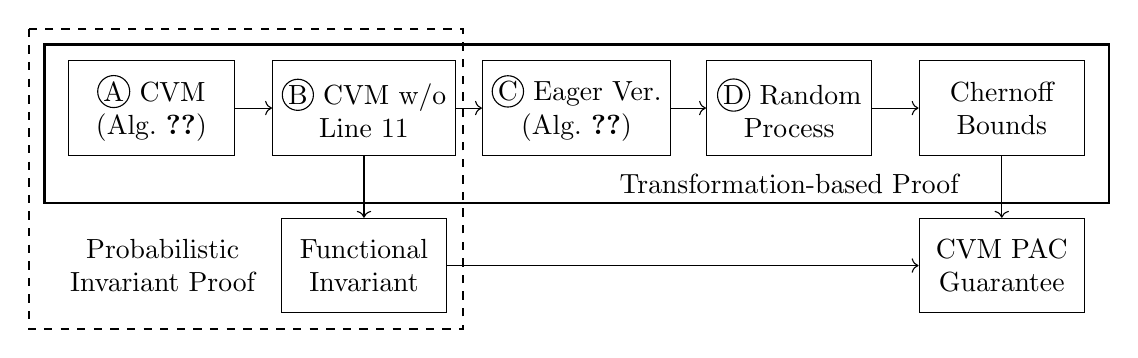
\begin{tikzpicture}[node distance=2.7cm, auto]

    % Define nodes
    \node (A) [draw, rectangle, minimum width=2.1cm, minimum height=1.2cm, align=center] {\circled{A} CVM \\ (Alg.~\ref{alg:cvm})};
    \node (B) [draw, rectangle, minimum width=2.1cm, minimum height=1.2cm, align=center, right of=A] {\circled{B} CVM w/o\\ Line 11};
    \node (C) [draw, rectangle, minimum width=2.1cm, minimum height=1.2cm, align=center, right of=B] {\circled{C} Eager Ver.\\(Alg.~\ref{alg:cvm_simul})};
    \node (D) [draw, rectangle, minimum width=2.1cm, minimum height=1.2cm, align=center, right of=C] {\circled{D} Random \\ Process};
    \node (E) [draw, rectangle, minimum width=2.1cm, minimum height=1.2cm, align=center, right of=D] {Chernoff \\ Bounds};

    \node (C') [draw, rectangle, minimum width=2.1cm, minimum height=1.2cm, align=center, below of=B, node distance = 2.0cm] {Functional\\Invariant};

    \node (pac) [draw, rectangle, minimum width=2.1cm, minimum height=1.2cm, align=center, below of=E, node distance = 2.0cm] {CVM PAC\\ Guarantee};

    \draw[thick] ($(A.north west) + (-0.3,0.2)$) rectangle ($(E.south east) + (0.3,-0.6)$);
    \node[anchor=south] at ($(D.south) + (0.0,-0.6)$) {Transformation-based Proof};

    \draw[dashed,thick] ($(A.north west) + (-0.5,0.4)$) rectangle ($(C'.south east) + (0.2,-0.2)$);
    \node[anchor=south,align=center] at ($(C'.west) + (-1.5,-0.45)$) {Probabilistic\\Invariant Proof};


    % Draw arrows
    \draw[->] (A) -- (B);
    \draw[->] (B) -- (C);
    \draw[->] (B) -- (C');
    \draw[->] (C) -- (D);
    \draw[->] (D) -- (E);
    \draw[->] (E) -- (pac);
    \draw[->] (C') -- (pac);

\end{tikzpicture}
\end{center}
\caption{An overview of the two formalized proof approaches for the CVM algorithm.}\label{fig:proof_overview}
\end{figure}

\subsection{A Bridging Transformation}
\begin{algorithm}[t]
	\caption{Modified CVM algorithm with independent coin flips. The function last{\textunderscore}index returns the index of the last occurrence of an element in the sequence, before the current iteration.}\label{alg:cvm_simul}
	\begin{algorithmic}[1]
  \Require Stream elements $a_1,\dots,a_l$, $0 < \varepsilon$, $0 < \delta < 1$.
  \Ensure A cardinality estimate $R$ for set $A = \{ a_1,\dots,a_l \}$ such that $\prob \left( |R - |A| | > \varepsilon |A| \right) \leq \delta$
  \State $\chi \gets \{\}, k \gets 0, n = \ceil*{\frac{12}{\varepsilon^2} \ln{(\frac{6l}{\delta})} }$
  \State $b[i,j] \getsr \Ber(1/2)$ for $i,j \in \{1,\cdots,l\}$ \Comment perform $l^2$ unbiased independent coin flips
  \For{$i \gets 1$ to $l$}
    \If{$b[i,1]=b[i,2]=\cdots=b[i,k]=1$} \Comment insert $a_i$ if first $k$ flips are $1$s.
      \State $\chi \gets \chi \cup \{a_i\}$
    \Else
      \State $\chi \gets \chi - \{a_i\}$
    \EndIf
    \If{$|\chi| = n$} \Comment if buffer $\chi$ is full
      \State $\chi \gets \{a \in \chi \;|\; b[\textrm{last{\textunderscore}index}(a),k+1] = 1\}$ \Comment keep elems.~whose $k+1$-th flip is $1$
      \State $k \gets k+1$
    \EndIf
    %\If{$|\chi| = n$}
    %  \State \Return $\bot$
    %\EndIf
  \EndFor
  \State \Return $2^k |\chi|$ \Comment estimate cardinality of $A$
  \end{algorithmic}
\end{algorithm}

Let us consider algorithm \circled{B} in a state where $k$ subsampling steps have been performed, i.e., $p = 2^{-k}$.
The algorithm would perform a coin flip lazily with probability $p$ when it encounters the next stream element.
The transformation \circled{C} is shown in \cref{alg:cvm_simul}, and we prove that it computes precisely the same distribution as \circled{B}.
In \circled{C}, we eagerly perform a fixed number of coin flips for each sequence element at the beginning.
Now, each element is put into the state $\chi$, whenever the first $k$ coin flips associated with the sequence element are all $1$s.
This happens exactly with probability $2^{-k}$, which means the behaviour of the algorithm is unchanged from \circled{B}.
Similarly, in the subsampling operation, only those elements whose $k+1$-th associated coin flip is $1$ are kept; the operation $p \mapsto \frac{p}{2}$ is replaced with $k \mapsto k+1$.
This again preserves the behaviour of \circled{B} that each element is discarded independently with probability $1/2$.

It is easy to show for \circled{C} that the coin flips are independent, and that the set of elements in $\chi$ in any state are exactly those stream elements for which the first $k$ entries of their associated coin flips are $1$.
The final random process $\circled{D}$ directly computes the final set of elements in $\chi$ after the stream, taking $K$ as a fixed parameter; one relates \circled{C} to \circled{D} by:
\[ \prob_{\circled{C}}(k = K \land \chi = X)  \leq \prob_{\circled{D}_K}(\chi = X)\]
for fixed values of $K$ and $X$.
To see how tail bounds can be derived from this inequality, let us first consider the failure event where the algorithm \circled{C}'s estimate exceeds the desired estimation interval and it ends with some fixed value $k = K$.
Using \circled{D}, this can be bounded using a Chernoff bound for the probability that the number of stream elements whose associated coin flips start with $K$ $1$s is outside $2^{-K} |A| (1 \pm \varepsilon)$.
Now, we can take a union bound over all the possible values $K$ to establish a global bound for the failure event in \circled{C}.
This is explained in more detail by Chakraborty et al.~\cite{chakraborty2023}.

%Like, we did in \cref{sec:invariants}, we ignore the second check, whether the subsampling operation succeeded.
%As we explained there, the total variational difference between these two variants is $\frac{\delta}{2}$.
%
\subsection{Eager to Lazy Coin Flips}
A remaining question is how to formalize the transformation from \circled{B} to \circled{C}.
Our insight is that it is best to solve the problem backwards, i.e., we start with the modified algorithm \circled{C}, which performs all the coin flips in advance \emph{eagerly} and convert it back to \circled{B} which implicitly performs the coin flips \emph{lazily} at the point they are needed.

The main idea is to automatically push down the coin flips through the expression tree of \cref{alg:cvm_simul}.
To explain how this works, let us first define the \emph{sampling} function, i.e., let $f$ be a function that takes as argument a vector of coin flips indexed by $I$, then we can express the distribution of $f$ with respect to independent unbiased coin flips as:
\begin{isabelle_cm}
  sample\ f\ \isacharequal\ map{\isacharunderscore}pmf\ f\ {\isacharparenleft}prod{\isacharunderscore}pmf\ I\ {\isacharparenleft}\isasymlambda\isacharunderscore\isachardot\ bernoulli{\isacharunderscore}pmf \isacharparenleft\isadigit{1}/\isadigit{2}\isacharparenright\isacharparenright\isacharparenright
\end{isabelle_cm}
%For example, we could use our modified algorithm as $f$, with the index set $I = \{0, \ldots, l-1\} \times \{0, \ldots, l-1\}$.
The interesting fact is that we can distribute the sampling operation over composition:
\begin{observation}\label{o:sample_distrib} Let $f,g$ be functions consuming a set of coin flips (indexed by $I$), where $g$ also consumes the output of $f$, such that,
$f$ depends only on the coin flips indexed by $J \subseteq I$ and $g$ depends on the complement $I - J$, then:
\begin{isabelle_cm}
  sample\ \isacharparenleft\isasymlambda\isasymomega\isachardot\ g\ \isasymomega\ \isasymcirc\ f\ \isasymomega{\isacharparenright}\ \isacharequal\ sample\ f\ \isasymbind\ \isacharparenleft{\isasymlambda}x\isachardot\ sample\ \isacharparenleft\isasymlambda\isasymomega\isachardot\ g\ \isasymomega\ x\isacharparenright\isacharparenright
\end{isabelle_cm}
\end{observation}
By recursively applying the observation, we end up with elementary lookup operations, e.g., \isa{sample\ \isacharparenleft\isasymlambda\isasymomega\isachardot\ \isasymomega\ i\isacharparenright}, for which it is easy to see that it is just a coin flip, i.e., equal to \isa{bernoulli{\isacharunderscore}pmf\ \isacharparenleft\isadigit{1}/\isadigit{2}\isacharparenright}.
This lets us readily transform \circled{C} to \circled{B} and prove their distributions equivalent.

A detail that we have simplified here is that the split of the index sets, e.g., which coin flips $f$ depends on and which coin flips $g$ depends on, may be dynamic.
For example, when the algorithm increases the subsampling counter $k$, it will have read the corresponding row of coin flips.
This means we have a situation where the previous loop iteration communicates to the next loop iteration which coin flips it depends on using the state.
And the next loop iteration will indeed only read coin flips that were not read by the previous iteration.
%For the column index of the coin flips, this is based on the stream index, but for the row index of the coin flips, it is based on the state variable $k$.

To handle these situations we generalized \cref{o:sample_distrib} to allow for the case where the cut between the set of coin flips $f$ and $g$ depend on, may depend on the result of $f$.
%It is possible to express the above in a point-free manner using the reader monad.
%This is a deterministic monad, which provides a read operation to a global value, such as our set of coin flips.
%(In Haskell, the reader monad is commonly used to provide a fixed environment to algorithms, such as global configuration options, paths or command lines parameters~\cite{jones1995}.)
%
%\begin{isabelle_cm}
%\isacommand{datatype}\ \isacharparenleft{\isacharprime}c\isacharcomma\ {\isacharprime}a\isacharparenright\ reader{\isacharunderscore}monad\ =\ Reader\ {\isacharparenleft}run{\isacharunderscore}reader\isacharcolon\ \isacartoucheopen{\isacharprime}c\ \isasymRightarrow\ {\isacharprime}a\isacartoucheclose\isacharparenright)\isanewline
%\isanewline
%\isacommand{definition}\ bind{\isacharunderscore}rd\ \isacommand{where}\ {\isacartoucheopen}bind{\isacharunderscore}rd\ m\ f\ \isacharequal\ Reader\ \isacharparenleft{\isasymlambda}r\isachardot\ run{\isacharunderscore}reader\ {\isacharparenleft}f\ {\isacharparenleft}run{\isacharunderscore}reader\ m\ r\isacharparenright\isacharparenright\ r\isacharparenright\isacartoucheclose\isanewline
%\isacommand{definition}\ return{\isacharunderscore}rd\ \isacommand{where}\ {\isacartoucheopen}return{\isacharunderscore}rd\ x\ \isacharequal\ Reader\ \isacharparenleft{\isasymlambda}{\isacharunderscore}\isachardot\ x\isacharparenright\isacartoucheclose\isanewline
%\isacommand{definition}\ get{\isacharunderscore}rd\ \isacommand{where}\ {\isacartoucheopen}get{\isacharunderscore}rd\ x\ \isacharequal\ Reader\ id\isacartoucheclose
%\end{isabelle_cm}
%With the definition above, we can define our sampling function with respect to the reader monad, where the environment is the entire set of coin flips, which is now a monad morphism (from the reader monad to the Giry monad):
%\begin{isabelle_cm}
%  sample{\isacharunderscore}rd\ \isacharequal\ sample\ \isasymcirc\ run{\isacharunderscore}reader
%\end{isabelle_cm}



\section{Related Work}\label{sec:related_work}
\subsection{Algorithms for the Distinct Elements Problem}
It is important to note that there are several practical solutions for the distinct elements problem.
The first solution was presented by Flajolet~\cite{flajolet1985} in 1985; however, like many other authors~\cite{flajolet2007,heule2013,pettie2021}, his solution makes the assumption that a fixed hash function can be regarded as a fully random function.
Alon et al.~\cite[Section 2.3]{alon1999} presented an easy remedy, which does not require such unmotivated model assumptions.
Their algorithm just relies on keeping track of the maximum of the hash values of the stream elements, where the hash function must be chosen uniformly from a pairwise independent family.

Later, Bar-Yossef et al.~\cite{baryossef2002}, Kane et al.~\cite{kane2010} and B\l{}asiok in 2020~\cite{blasiok2020} improved on the solution by Alon et al.
For example, Bar-Yossef et al.\ present a solution (Algorithm~3 in their work) with a space-complexity of $\bigo(\ln (\delta^{-1}) (\varepsilon^{-2}(\ln(\varepsilon^{-1})+\ln b) + b)))$, which can be implemented in practice.
This is slightly better than the CVM algorithm which requires $\bigo(\varepsilon^{-2} \ln (\delta^{-1}l) b)$. In particular, there is no dependency on the length of the stream $l$.
The more recent and more sophisticated solution by B\l{}asiok is space-optimal, with a space complexity of $\bigo(\varepsilon^{-2} \ln (\delta^{-1}) + b)$.
We~\cite{karayel2023} presented a version of the latter that preserves monotonicity and supports the merge-operation, which enables its use in distributed settings, such as Map-Reduce pipelines~\cite{dean2010}.
It should be noted that these recent algorithms are mostly of theoretical interest, as the constants, as well as the implementation complexity, are rather large.
What makes the CVM algorithm unique is its simplicity and the fact that it does not rely on hashing, which may enable more general use-cases than the traditional algorithms.

The aforementioned hash-based algorithms are biased; Flajolet et al.~\cite{flajolet1985} points this out and also provides bounds on the distance between the expected result and the cardinality of the stream.
Most authors do not discuss the matter of bias but it is not hard to show.
One issue, for example, is that the usual method to amplify the accuracy of these algorithms is using the median, which does not preserve expectations.
In the context of query processing, unbiasedness has been discussed~\cite[Section 2.1]{haas1995}, but we could not find any similar discussion for the distinct elements problem in the streaming model.

\subsection{Probabilistic Invariants and Formalization}
As far as we know, probabilistic invariants have not been used to establish exponentially decreasing tail-bounds.
However, it is fairly common to use recursive analysis techniques to establish results about expectations or variance of random variables, such as their run-time~\cite[Section 1.4]{motwani1995}.
This is easy due to the linearity of expectations and---for independent random variables---linearity of variances.
A simple example is the Morris counter~\cite{morris1978} or the expected run-time of the quick-sort algorithm~\cite[Section 2.5]{mitzenmacher2005}.

There is also research on the (automated) analysis of loop invariants, for probabilistic loops, using their characteristic functions~\cite{batz2023, mciver2005}.
This approach works by establishing the limiting distribution of the state of the loop.
De Medeiros et al.~\cite[Section 3.2]{demedeiros2024} also establish methods to derive limiting distributions of probabilistic loops.
Our approach differs from these techniques by avoiding computation of the distribution, which, we think, is infeasible for the CVM algorithm.
Instead, we investigate invariants of classes of functions of the distributions, which are relevant for the analysis.
There is research on automated evaluation of moments for restricted classes of loops which contain only polynomial assignments and no branches~\cite{bartocci2019,kofnov2022}.
However, these methods do not extend to algorithms with branches or, more generally, algorithms which contain discrete operations.

Finally, verification of randomized algorithms has been tackled by various authors using various proof assistants~\cite{bosshard2024,demedeiros2024, eberl2020,gopinathan20,hurd03, Probabilistic_Prime_Tests-AFP, tan2024}.
The most closely related efforts are our mechanizations of frequency moments algorithms~\cite{karayel2022, karayel2023}.
The functional invariant proof technique we introduce here should be applicable in any higher-order setting.


\section{Conclusion}\label{sec:conclusion}
We presented the first formalization of the CVM algorithm using Isabelle/HOL.
Central to our formalization is a novel invariant-based proof technique to establish exponentially decreasing tail-bounds for randomized algorithms, which is inspired by our alternative analysis of the CVM algorithm via the Cram\'{e}r--Chernoff method; comparing our approach against the original proof by Chakraborty et al.~\cite{chakraborty2023} shows that our technique yields a considerably shorter formalization (with \locnew~vs.~\locold~lines).
Interestingly, our technique also readily generalized to a new CVM variant with stronger properties (totality and unbiasedness)---we formalized this latter version using the same invariant, together with a new library of results for negative association.
In future work, it would be interesting to formalize other variations of subsampling for CVM.

Our novel technique can be summarized by the following two steps:
\begin{enumerate}
\item Find functions of the state of the algorithm, for which it is possible to establish upper bounds of their expectation recursively. 
\item Use those bounds to establish tail bounds on the result of the algorithm.
\end{enumerate}
However, we would like to note that, we do not yet have good further examples, where our approach can be applied to. (It is easy to construct artificial examples.)
This also means that our definition of the method may require refinement.
Another issue is that we do not have general strategies to identify the functionals to consider.
Identification of realistic applications for this new method is an interesting avenue for future work.


%%
%% Bibliography
%%

%% Please use bibtex,

\bibliography{main}

\end{document}
